\section{Metalsmith}
\label{sec:metalsmith}

Compared to the already described static site generators, \emph{Metalsmith} is to be considered the youngest project.
It might also be the most radical project, as it was designed to consist of \emph{nothing but plugins} \cite[31]{dhillon2016}. Therefore, in terms of still being a static site generator, it tries hard to push the limits much further than previously mentioned Jekyll and Hexo.

\subsection{History}
\label{sec:metalsmith-history}
Initially developed by \emph{Segment}\footnote{\url{https://segment.com} -- Segment's website.} for their internal needs, such as \emph{documentation, help} and \emph{blog pages} \cite{Metalsmith2015buildingblocks}, Metalsmith was finally open-sourced and made publicly available around February 2015 -- its commit history on GitHub dates back to February 4\textsuperscript{th}, 2014. Most of the commits at that time were published by \emph{Ian Storm Taylor}, co-founder of Segment, although his contribution to the project ends after releasing \emph{v2.1.0} on September 24\textsuperscript{th}, 2015\footnote{\url{https://github.com/segmentio/metalsmith/commits/master?author=ianstormtaylor} -- Contributions of Ian Storm Taylor to the Metalsmith repository on GitHub.} at the moment.

Like Hexo, Metalsmith's repository completely consists of JavaScript code, as its developers also were unsatisfied with the then existing static site generators. According to Chris Sperandio, the Metalsmith developers desired pure flexibility for their ``wide array of use cases'', while other frameworks all asked for a certain structure on the content \cite{Metalsmith2015buildingblocks}.

\subsection{Technology}
\label{sec:metalsmith-technology}
Since Metalsmith consists of only plugins, specifically written for this very framework, there is no real standard setup provided. Although there are a few tutorials and best practices listed in its GitHub repository \cite{MetalsmithRepository}, as well as in a repository called ``\emph{awesome-metalsmith}''\footnote{\url{https://github.com/metalsmith/awesome-metalsmith} -- ``Awesome'' Metalsmith resources list.}, the initial dive-in might scare a few people away, since Metalsmith might not be as well documented as the previously mentioned frameworks. Moreover, most developers seem to experience a very steep learning curve at first, given the amount of customization options and the requirements for understanding the blog engine~infrastructure \cite[31]{dhillon2016}.

\subsubsection{Advantages}
Every developer is able to shape Metalsmith exactly to his/her needs, once he knows about the basic usage. It ships with a CLI, as well as a JavaScript API, where the ``real hacking'' is possible. The CLI gets easily configured via a \texttt{metalsmith.json} file, stored in the project directory. It consists mainly of general project configurations, placed in the object's root, as well as an array of used plugins, respectively combined with their configuration.

It neither contains a pre-installed template engine, nor any other pre-processing tools, like Sass or Less. However, the available plugins support most of them to a satisfying extent. As an example, the metalsmith-layouts plugin is a wrapper for \emph{Consolidate.js}, which per se acts as a wrapper for the most common template engines\footnote{\url{https://github.com/tj/consolidate.js\#supported-template-engines} -- Consolidate.js-supported template engines on GitHub.}. Therefore, the developer is able to select the tools based on his/her preferences and may initialize a project from scratch, without needing to clean up any pre-installed demonstration files first.

Using the built-in JavaScript API, it is also possible to invoke the needed modules programmatically, which is one of the core topics of this Thesis.

\subsubsection{Disadvantages}
So much freedom in designing a project may also cause some dangers. In this case, one of the most crucial things is the arrangement of plugins in the configuration. Since Metalsmith acts as a streaming build system, every transformation of the content must happen at its time to not interfere with any upcoming plugins. This is especially important when a plugin might alter the underlying code in a way, that a following plugin becomes useless, as it might not be able to succeed in its predefined task. \emph{Andy Jiang} gives a good example about a sample structuring of Metalsmith plugins on the Segment blog \cite{Metalsmith2015technicaldocumentation}.

As an example, Program \ref{list:metalsmith} shows one bold example of misconfiguration (see line 16):

\begin{program}
%% Update line no. above, if code changes
\caption{config.js}
\label{list:metalsmith}
\lstinputlisting[language=JavaScript]{chapters/02-state-of-the-art/_support/metalsmith.js}
\end{program}

%% Screenshot of npms.io for search query metalsmith static assets
\begin{figure} % h-ere, t-op, b-ottom, p-age
    \centering
    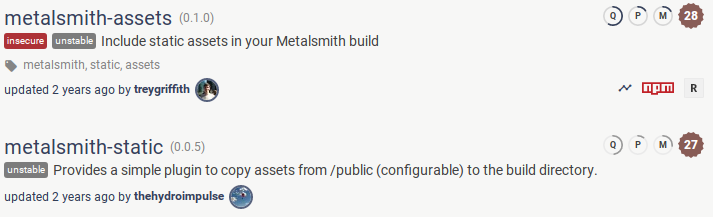
\includegraphics[width=0.9\textwidth]{metalsmith-static-plugins.png}
    \caption{A screenshot showing some of the results for the search query ``\emph{metalsmith static assets}'' on \url{https://npms.io}. Both of the shown entries describe an identical mode of operation within the Metalsmith build pipeline.\\
    Also notice the very unstable \emph{semver} versions: \emph{0.1.0} and \emph{0.0.5}.}
    \label{fig:metalsmith-plugins}
\end{figure}
%

Moreover, the available plugins may seem as not as popular as the plugins from Hexo, given the average amount of stars received on GitHub. This might be due to the often missing maintainance, or simply because of the fact, that there seem to be multiple plugins for one single task (see Fig. \ref{fig:metalsmith-plugins}).
